\Chapter{Contexte et travaux connexes}\label{chap:revue}


\section{Web sémantique et logique descriptive}
\label{sec:dl}

\subsection{Graphes de connaissance}

% À déplacer vers l'INtroduction ??

%Un graphe de connaissance permet de représenter des données de manière structurée. Il consiste en un ensemble d'objets du monde réel, appellés \textit{entités}, reliés entre eux par des \textit{relations}.

%On se donne $\Ent$ un ensemble d'entités, et $\Rel$ un ensemble de relations. En pratique, chaque entité ou relation est représentée par un identifiant unique, l'URI (\textit{Universal Resource Identifier}).

%Un graphe de connaissance 

Un graphe de connaissance est une collection structurée de données permettant de représenter des informations, ou des \textit{faits}, sur le monde réel. La définition exacte d'un graphe de connaissance varie d'un auteur à l'autre \cite{ehrlinger2016towards}; parmi les caractéristiques fréquemment retenues, on notera l'interrelation des données et le caractère multi-relationnel, l'existence d'une sémantique formelle et de mécanismes de raisonnement, ou parfois une certaine taille critique. Les paragraphes suivants visent à définir et expliciter ces différentes propriétés.


\paragraph{Concepts de base}

Dans ce travail, on adopte une définition très générale d'un graphe de connaissance vu comme un ensemble d'entités liées entre elles par des relations. Pour un ensemble d'entités $\Ent$ et un ensemble de relations $\Rel$, un graphe de connaissance est simplement un ensemble de triplets $\KG \subseteq \Ent \times \Rel \times \Ent$. Si $(h, r, t)$ est un triplet du graphe, alors l'entité $h$ est reliée à l'entité $t$ par la relation $r$; dans ce cas, on dit que $h$ est le \textit{sujet} du triplet, et $t$ son objet. Le choix des notations s'explique par l'anglais, $h$ désignant la tête (\textit{head}) et $t$ la queue (\textit{tail}) du triplet. 
% Pour un graphe de connaissance, on parle fréquement de données \textit{multi-relationnelles} pour indiquer que les entités

En pratique, lorsqu'on parle de graphe de connaissance, on s'attend à quelques restrictions supplémentaires. D'une part, les données d'un graphe de connaissance doivent être \textit{multi-relationnelles}, c'est-à-dire qu'il existe plusieurs relations possibles entre les entités ($| \Rel | > 1$); d'autre part, les entités sont reliées mutuellement entre elles. Ainsi, un système reliant des fichiers à des méta-données textuelles ne saurait être qualifié de graphe de connaissance; dans un graphe de connaissance, les objets d'un triplet sont, au moins pour partie, sujets d'autre triplets, et le graphe forme donc un réseau d'entités interconnectées. 


Le format dominant pour représenter un tel graphe est le format RDF, pour \textit{Resource Description Framework} \cite{cyganiak14}. En RDF, les entités sont de deux types : soit des identifiants, soit des littéraux. Les identifants, ou URI, pour \textit{Uniform Resource Identifier}, sont simplement des chaînes de caractères qui désignent des ressources du monde réel : lieux, personnes, documents, etc. %Il est courant de regrouper des identifiants au sein d'un \textit{vocabulaire} commun
RDF n'impose pas de mécanisme pour relier les URI aux entités qu'elles désignent. 
Les littéraux permettent de représenter des valeurs fixes : nombres, textes, booléens, dates, sommes d'argent. Contrairement aux identifiants, l'interprétation des littéraux est définie une fois pour toutes; la manière d'interpréter un littéral est indiquée par son \textit{format} (parfois appelé \textit{datatype} en anglais). Par exemple, le littéral \texttt{1901-01-28\^{}\^{}xsd:date} est constitué de la valeur \texttt{1901-01-28} au format \texttt{xsd:date}, et s'interprète de manière unique comme la date du 28 janvier 1901.

Un \textit{vocabulaire} est un ensemble d'URI, présentant une certaine cohérence. Les URI d'un même vocabulaire partagent quasi-systématiquement une racine commune, que l'on peut alors abréger par un \textit{préfixe}. Ainsi, toutes les URI du vocabulaire standard RDF commencent par \texttt{http://www.w3.org/1999/02/22-rdf-syntax-ns\#}, que l'on abrège en \texttt{rdf:}. Ainsi, les URI \texttt{http://www.w3.org/1999/02/22-rdf-syntax-ns\#type} et \texttt{http://www.w3.org/1999/02/22-rdf-syntax-ns\#Property} sont abrégées en \texttt{rdf:type} et \texttt{rdf:Property}, respectivement. 


% De la même manière, les entités de DBpédia sont regroupées dans un vocabulaire commun, dont le préfixe usuel est \texttt{dbr} (abrégé de \texttt{http://dbpedia.org/resource/}) : ainsi, \dbr{Montréal} ou \dbr{Pablo\_Picasso} désignent des entités de DBpédia.

% DBpédia

\paragraph{Un exemple : DBpédia}

Il existe de nombreux graphes de connaissance publics; certains sont restreints à un domaine spécifique, comme WordNet \cite{miller1998wordnet}, d'autres sont généraux, comme YAGO \cite{suchanek2008yago} ou Wikidata \cite{vrandevcic2014wikidata}. Parmi ces graphes de connaissances généralistes, l'un des plus notables est DBpédia \cite{auer2007dbpedia}, sur lequel on s'appuiera dans toute la suite de ce travail, dans sa version anglaise. Les données de DBpédia sont obtenues de manière automatique en aggrégeant différentes sources issues de Wikimédia, en premier lieu desquelles les infoboîtes de Wikipédia. Le cœur de DBpédia est son système d'extraction, qui convertit Wikipédia en un ensemble de triplets RDF à l'aide de différentes heuristiques; cet extracteur s'appuie essentiellement sur les infoboîtes de Wikipédia, des encarts constituées de paires clé-valeur et dont le format est relativement uniformisé à l'échelle de Wikipédia. Outre les infoboîtes, l'extracteur utilise également les liens de redirection et de désambiguïsation, les catégories des pages, les éventuelles informations de géolocalisation, etc. À cet extracteur s'ajoutent différentes procédures pour nettoyer et uniformiser les résultats, ainsi que pour aggréger des données provenant d'autres sources. DBpédia fournit également un point d'entrée pour effectuer des requêtes sur le graphe\footnote{\href{https://dbpedia.org/sparql}{dbpedia.org/sparql}}.

Les entités de DBpédia sont regroupées au sein d'un vocabulaire \texttt{http://dbpedia.org/resource/}, généralement abrégé en \dbr{}. Le voisinage d'une entité donnée \dbr{<Nom de l'entité>}, c'est-à-dire les triplets dont cette entité est le sujet ou l'objet, peut être consulté en ligne à l'adresse \href{http://dbpedia.org/page/<Nom de l'entité>}{dbpedia.org/page/<Nom de l'entité>}. Les relations et les classes de DBpédia font elles parties du vocabulaire \texttt{http://dbpedia.org/ontology/}, abrégé en \dbo{}.


DBpédia contient à l'heure actuelle 1 300 relations et 4,2 millions d'entités pour un total de 56,5 millions de triplets. Les entités sont réparties selon 655 types, dont les plus fréquents sont les personnes (\dbo{Person}), les lieux (\dbo{Place}), les espèces (\dbo{Species}), les événements (\dbo{Event}), les œuvres (\dbo{Work}, entendu au sens large et incluant livres, films, etc.), les organisations (\dbo{Organisation}). Comme les données de DBpédia sont extraites automatiquement de Wikipédia et que Wikipédia est modifié régulièrement, le graphe DBpédia évolue lui aussi régulièrement.


\paragraph{Typologie des relations} 

Il est utile de détailler les propriétés que peuvent avoir les relations dans un graphe de connaissance, et en premier lieu leur caractère symétrique ou antisymétrique :
\begin{itemize}
    \item une relation $r$ est \textbf{symétrique} si $\rel{t}{r}{h}$ est vérifiée dès que $\rel{h}{r}{t}$ est vérifiée. Par exemple, la relation \texttt{owl:sameAs}, qui indique que deux URI correspondent à la même entité, est naturellement symétrique. Plus généralement, toutes les relations qui impliquent une équivalence ou une réciprocité sont symétriques, comme \dbo{spouse} ou \dbo{colleague};
    \item à l'inverse, une relation $r$ est \textbf{antisymétrique} si $\rel{h}{r}{t}$ et $\rel{t}{r}{h}$ ne peuvent jamais être vérifiées simultanément. C'est le cas, en pratique, de la relation \texttt{rdfs:subClassOf} et de la plupart des relations hiérarchiques comme \dbo{isPartOf} ou \dbo{parent};
\end{itemize}
Une relation peut très bien n'être ni symétrique, ni antisymétrique. La relation \dbo{influenced}, qui marque l'influence intellectuelle d'une personne sur un autre, est parfois mutuelle (pensons par exemple à Russell et Wittgenstein, ou Beauvoir et Sartre) et parfois non.

On peut également classer les relations selon les cardinalités relatives de leurs sujets et de leurs objets :
\begin{itemize}
    \item une relation \textbf{\textit{one-to-many}} (de un à plusieurs, en français) lie chaque sujet à plusieurs objets : par exemple, pour la relation \dbo{isAuthorOf}, un auteur est relié à chacune de ses œuvres, tandis qu'une œuvre n'a en général qu'un seul auteur;
    \item à l'opposé, une relation \textbf{\textit{many-to-one}} (de plusieurs à un) lie plusieurs sujets à un même objet; c'est le cas de la relation \texttt{foaf:gender} qui, dans DBpédia, relie un million et demi de sujets à seulement trois objets (\texttt{"male"}, \texttt{"female"} et \texttt{"non-binary"});
    \item une relation \textbf{\textit{one-to-one}} (un pour un) relie un sujet à un unique objet, et réciproquement. On peut penser à la relation qui unit un pays à sa capitale (\dbo{capital}), ou une entité à son label (\texttt{rdfs:label});
    \item enfin, une relation \textbf{\textit{many-to-many}} relie un sujet à plusieurs objets, et un objet à plusieurs sujets. Cette catégorie comprend par exemple la relation \dbo{influenced} citée plus haut : en général, un artiste ou un penseur est influencé par plusieurs personnes, et en influence d'autres à son tour;
\end{itemize}
La caractérisation ci-dessus ne constitue pas une classification formelle des relations, et la frontière entre ces différents types de relation est parfois floue. Examinons par exemple la relation \texttt{rdf:type}, fondamentale pour le reste de ce travail, qui associe à chaque entité les types auxquels il appartient. En général, une entité a plusieurs types : dans DBpédia, \dbr{Gaston\_Miron} possède à la fois les types \dbo{Poet}, \dbo{Person}, \dbo{Agent} et \texttt{owl:Thing}. Réciproquement, de nombreuses entités sont liées à chacun de ces types. On serait donc tenté de catégoriser la relation \texttt{rdf:type} comme une relation \textit{many-to-many}. Pourtant, les effectifs d'un côté et de l'autre sont très déséquilibrés : là où une entité possède au plus sept types distincts, un type est relié en moyenne à X entités, ce qui apparenterait davantage la relation \texttt{rdf:type} comme une relation \textit{many-to-one}. % Dans le cadre de ce travail, il est plus pertinent de considérer \texttt{rdf:type} comme une relation \textit{many-to-one}.

\subsection{Ontologies et logique descriptive}

Introduction : axiomes logiques permettant de décrire des classes, des relations, des interactions entre les deux, des restrictions des contraintes, etc.

% Présentation

La logique descriptive est un terme général englobant une famille de systèmes logiques, dont l'usage est précisément de pouvoir décrire des données multi-relationnelles. 
Le choix d'un système logique nécessite un compromis entre deux aspects : l'expressivité et la calculabilité. L'expressivité désigne la capacité à modéliser des situations complexes; la calculabilité concerne 

On souhaite en effet avoir une expressivité suffisante pour être capable de modéliser logiquement des situations complexes; toutefois, augmenter l'expressivité d'une logique a pour conséquence d'accroître le temps de calcul pour effectuer des raisonnements.


La logique descriptive manipule trois types d'éléments : des entités (ou \textit{individus}), des relations, et des concepts. Les concepts sont des ensembles d'entités, et les relations décrivent des liens entre deux entités. Entités, relations et concepts peuvent être combinés entre eux pour former des \textit{axiomes}; les types de combinaisons possibles varient selon la logique descriptive choisie

une ontologie est alors simplement un ensemble d'axiomes, chacun d'entre eux devant être vrai dans la situation décrite.

Ici, on présentera uniquement les axiomes utilisés dans la suite du mémoire; pour une description plus complète, on pourra consulter \cite{krotzsch2013description}. 

Subsumption 
\begin{equation}
    \texttt{Athlète} \sqsubseteq \texttt{Personne}
\end{equation}


On peut également définir un concept singleton, c'est-à-dire un concept constitué d'un seul individu :
\begin{equation}
    \{ \texttt{Canada} \}
\end{equation}

Équivalence
\begin{equation}
    \texttt{Personne} \equiv \texttt{Humain}
\end{equation}

Disjonction
\begin{equation}
    \texttt{Animal} \equiv \texttt{Vertébré} \sqcup \texttt{Invertébré}
\end{equation}

Conjonction
\begin{equation}
    A \sqcap B
\end{equation}

Concept universel
\begin{equation}
    \top
\end{equation}

Complémentaire
\begin{equation}
    A^-
\end{equation}

Existentiel
\begin{equation}
    \exists \texttt{écrit}.\texttt{Poème}
\end{equation}

% Existentiel 2
\begin{equation}
    \texttt{Poète} \equiv \texttt{Personne} \sqcap \exists \texttt{écrit}.\texttt{Poème}
\end{equation}


% Sémantique ? --> pas nécessaire ici / Inférence, raisonnement

% Taxonomie, ontologie
Dans la suite, on désignera par ontologie n'importe quel ensemble d'axiomes; par taxonomie, un ensemble d'axiomes de subsumption

% OWL

% Plongements de graphe

\section{Extraction automatique d'ontologie et de taxonomie}

% Non ça ça va dans la section 'Problématique' : Constuire une ontologie manuellement est coûteux. Le graphe est dynamique et les données changent bla bla

Le problème d'extraction d'axiomes logiques n'est pas nouveau et prend des formes très variées. Dans le cas général, on cherche soit à apprendre une ontologie à partir de zéro (ref), soit à étendre une ontologie existante en construisant de nouveaux axiomes (ref). Un sous-problème fréquent est l'extraction de \textit{taxonomie} : il s'agit alors d'extraire uniquement des axiomes de subsumption, c'est-à-dire ayant la forme $A \sqsubseteq B$, afin d'obtenir une hiérarchie sur les concepts. Si on autorise ces concepts à prendre la forme d'axiomes plus complexes, on parlera d'extraction de taxonomie \textit{expressive}. 

On peut distinguer deux grandes familles de méthodes, selon la source des données utilisées : les méthodes basées sur le texte, et les méthodes basées sur un graphe de connaissance. Étant donné la très large disponibilité de corpus textuels étendus (et particulièrement en langue anglaise), les méthodes utilisant le texte sont aujourd'hui les plus fréquentes, et se concentrent particulièrement sur l'extraction de taxonomie. Les méthodes basées sur le graphe ont toutefois leurs avantages : en particulier, elles peuvent fonctionner pour les graphes spécifiques à un domaine et pour lesquels il n'existe pas de données textuelles – c'est le cas notamment du domaine biomédical. Notons que l'émergence conjointe des plongements lexicaux (pour le texte) et des plongements vectoriels de graphe permet d'envisager une convergence de ces deux familles de méthodes.


\subsection{Extraction d'ontologies à partir d'un graphe}

Raisonneurs : permettent d'inférer de nouveaux faits. Partent d'axiomes existants et de règle de démonstration (donner un exemple, par ex modus ponens) pour produire de nouveaux axiomes. Toutefois, ils ne permettent pas de créer une ontologie de zéro puisqu'ils supposent des axiomes de départ. On pourrait envisager de construire manuellement des axiomes, et de les étendre mais les raisonneurs passent mal à l'échelle ne tournent pas nécessairement sur DBpédia

Bla bla extraction à partir de graphe
On présente d'abord les méthodes symboliques, qui utilisent les règles et le formalisme de la logique. Ces méthodes sont pour la plupart mal adaptées aux graphes de connaissances créés automatiquement ou semi-automatiquement, et ce pour deux raisons essentielles : d'une part, ces méthodes demandent beaucoup de ressources, et ne fonctionnent que sur des ontologies réduites; d'autre part, elles sont incapables de gérer correctement l'incertitude et le bruit qui caractérise ces graphes. 

\subsubsection{Méthodes symboliques}

Les méthodes symboliques constituent une première famille d'approches capables de construire de nouveaux axiomes à partir d'axiomes existants. Ces méthodes sont pour la plupart mal adaptées aux graphes de connaissances créés automatiquement ou semi-automatiquement, et ce pour deux raisons essentielles : d'une part, ces méthodes demandent beaucoup de ressources, et ne fonctionnent que sur des ontologies réduites; d'autre part, elles sont incapables de gérer correctement l'incertitude et le bruit qui caractérise ces graphes. On en présente succintement trois grandes familles dans les paragraphes qui suivent.

Les raisonneurs, comme Fact++ \cite{tsarkov2006fact++} ou Hermit \cite{glimm2014hermit}, appliquent des règles de démonstration pour déduire des axiomes nouveaux. Un exemple de ces règles de démonstration est le \textit{modus ponens}, qui consiste simplement en $P \land (P \implies Q) \vdash Q$ : si $P$ est vraie et $P$ implique $Q$, alors $Q$ est vraie. Ces raisonneurs peuvent être utiles pour vérifier si une ontologie donnée est consistante, mais ils ne peuvent pas réellement être utilisés pour l'extraction de taxonomie : 
d'une part, ils nécessitent une ontologie de départ; d'autre part, ce sont des méthodes \textit{déductives} et donc incapable d'inférer de nouvelles règles à partir des données; enfin, la complexité de calcul augmente rapidement, ce qui les rend inadaptés pour des ontologies de grande taille.

Une autre approche symbolique est la \textbf{programmation logique inductive} (ou ILP, pour \textit{Inductive Logic Programming}): il s'agit cette fois d'une méthode \textit{inductive}, c'est-à-dire qui produit de nouveaux axiomes à partir d'exemples. La programmation logique inductive part d'une série d'axiomes (la \textit{théorie préalable}) et d'exemples positifs et négatifs; elle cherche à produire de nouveaux axiomes qui sont vérifiés par les exemples positifs  mais pas par les exemples négatifs. De manière informelle, on se donne une propriété $P$, une théorie préalable vide, un ensemble d'exemples positifs $E^+=\{P(0), P(2), P(4), P(8) \}$ et $E^- = \{ P(1), P(3), P(5) \}$ – autrement dit, $0, 2, 4, 8$ vérifient $P$ et $1, 3, 5$ ne la vérifient pas\footnote{Exemple tiré de \cite{nienhuys1997foundations}.}. Alors, un exemple de théorie induite est donné par :
\begin{align}
    & \textrm{Si } P(x) \textrm{ est vraie, alors } P(x + 2) \textrm{ est vraie.} \\
    & P(0) \textrm{ est vraie.}
\end{align}
Cette théorie ne pourrait être obtenue par un raisonneur, car elle n'est pas une conséquence logique de $E^+$ et de $E^-$ : il s'agit simplement d'une théorie plausible étant donnée les faits observés. Pour obtenir des théories induites pertinentes, la programmation logique inductive nécessite donc un choix judicieux d'exemples positifs et négatifs. Comme pour les raisonneurs, les méthodes de programmation logique inductive passent difficilement à l'échelle pour les graphes de connaissance de grande taille (\hl{ref}). De plus, les données d'un graphe réel sont incomplètes et bruitées, une situation pas ou mal gérée par la programmation logique. 

Une troisième approche symbolique repose sur l'\textbf{analyse formelle de concept} (en anglais :  \textit{Formal Concept Analysis}).



\subsubsection{Méthodes statistiques}
% Apprentissage statistique
Statistical Schema Induction


% À partir de textes
% Traduction d'axiomes depuis le langage naturel
\subsection{Méthodes utilisant les plongements vectoriels de graphe}

Encore assez peu exploité

TIEmb

\subsection{Extraction de taxonomie à partir de texte}

Ressource la plus abondante : corpus textuels
L'approche dominante consiste à extraire des taxonomies à partir de texte. Dans ce domaine, on parle généralement d'\textit{hyperonymie} pour qualifier la subsumption. 
Cela implique notamment d'identifier les concepts parmi les mots du vocabulaire, de détecter des paires hyponyme-hyperonyme, et de filtrer ces paires.

\subsubsection{Utilisation de motifs lexico-syntaxiques}

Une première approche consiste à définir des motifs lexico-syntaxiques, appelés motifs de Hearst \cite{hearst1992automatic} (ou \textit{Hearst patterns}, en anglais), pour identifier les relations d'hyperonymie. Par exemple, le motif $NP \texttt{ \{, } NP \texttt{ \}* \{, \} or other } NP$ (où NP indique l'emplacement de noms) trouve une occurrence dans la phrase «\textit{Bruises, wounds, broken bones or other injuries}» et permet de déduire que «\textit{bruise}», \textit{wound}» et «\textit{broken bone}» sont des hyponymes de «\textit{injury}»\footnote{Exemple tiré de \cite{hearst1992automatic}}.
Ces motifs sont généralement définis à la main, et fixés pendant toute la durée de l'extraction. Toutefois, certaines approches apprennent de nouveaux motifs au cours de l'extraction \cite{snow2005learning, shwartz-etal-2016-improving}. Appliquées à des corpus textuels étendus, les méthodes basées sur des motifs de Hearst ont généralement une bonne précision \cite{roller-etal-2018-hearst}, mais un mauvais rappel \cite{wu2008automatically}, car la langue naturelle présente une grande variabilité et il est difficile de définir des motifs capable de couvrir tous les cas d'hyperonymie.

Les paires hyponyme-hyperonyme extraites sont ensuite filtrées, afin d'éliminer les éventuelles erreurs d'extraction. Dans sa forme la plus simple, le filtrage consiste simplement à compter le nombre d'occurrence de chaque paire, et de définir un seuil minimal. En faisant cela, on pénalise toutefois les mots rares au détriment des mots fréquents : par exemple, il est plus probable d'extraire la paire \textit{(France, pays)} que \textit{(France, république)}, simplement parce que «pays» est un terme plus commun que «république». Pour résoudre ce problème, \cite{turney2001mining} utilise la PPMI (\textit{Positive Pointwise Mutual Information}, ou information mutuelle ponctuelle positive) entre deux termes. Si $w(x, y)$ désigne le nombre d'occurrences d'une paire $(x, y)$ dans les résultats d'extraction, et $W$ le nombre total de paires extraites, on peut définir une fréquence d'extraction $p(x, y) = w(x,y) / W$ pour la paire $(x, y)$; pour le terme $x$, on définit également une fréquence d'apparition en tant qu'hyponyme : $p^-(x) = \sum_y w(x, y) / W$ et en tant qu'hyperonyme : $p^+(x) = \sum_y w(y, x) / W$. La PPMI est alors calculée selon la formule :
\begin{equation}
    PPMI(x, y) = \max \left(0, \log\frac{p(x, y)}{p^-(x)p^+(y)} \right)
\end{equation}

La PPMI permet de résoudre le problème soulevé plus haut : on aura certes toujours $p(\textrm{France}, \textrm{pays}) > p(\textrm{France}, \textrm{république})$, mais également $p^+(\textrm{pays}) > p^+(\textrm{république})$, et donc normalement une PPMI comparable pour les deux paires \textit{(France, pays)} et \textit{(France, république)}.

Enfin, \cite{roller-etal-2018-hearst} propose de lisser les valeurs de PPMI obtenues en réduisant la dimension de la matrice de PPMI avec une SVD tronquée. Cela donne une représentation de rang faible des mots, qui permet alors de décider si deux mots sont hyperonymes l'un de l'autre, même si la paire exacte n'a pas été vue sur le corpus d'entraînement.

% Pour améliorer ce rappel, le plus simple est parfois d'améliorer la taille du corpus : (ref) a montré qu'utiliser un ensemble restreint de motifs sur des corpus très étendus permet une bonne extraction. Une autre solution consiste à apprendre de nouveaux motifs au cours de l'extraction \cite{snow2005learning, shwartz-etal-2016-improving}.

\subsubsection{Méthodes distributionnelles, méthodes à plongement}

Les méthodes distributionnelles reposent sur l'«hypothèse d'inclusion distributionnelle» (ou DIH, pour \textit{Distributional Inclusion Hypothesis}) \cite{geffet2005distributional} : si le terme A est un hyperonyme du terme B, alors les contextes dans lesquels B apparaît forment un sous-ensemble des contextes dans lesquels A apparaît. Le contexte d'un mot peut être les $2N$ mots adjacents au sein du corpus ($N$ mots précédents et $N$ mots suivants), ou les éléments voisins (parents ou enfants) au sein d'un arbre de dépendance \cite{shwartz-etal-2017-hypernyms}.
Intuitivement, cette hypothèse signifie que l'on peut remplacer les occurrences de B par A tout en gardant un texte valide.

Pour mettre en pratique cette idée, ces méthodes construisent une représentation vectorielles des termes; on peut alors évaluer si un terme A est un hyperonyme d'un terme B en utilisant une fonction de classification, qui combine les représentations de A et de B et prédit le résultat. 


\paragraph{Extraction des concepts}

L'extraction de taxonomie à partir de texte suppose deux étapes : d'abord, identifier, parmi tous les termes du corpus, ceux qui ceux qui constituent des concepts et qui sont donc impliquées dans des relations d'hyperonymie; ensuite, identifier les relations d'hyperonymie entre ces concepts. Les méthodes basées sur des motifs de Hearst effectuent simultanément ces deux étapes; ce n'est pas le cas des méthodes distributionnelles, qui supposent une étape préalable d'\textit{extraction des concepts}. Dans certains cas, les concepts sont considérés comme des données d'entrée, et l'enjeu est simplement de les ordonner hiérarchiquement. Autrement, il est nécessaire de filtrer le corpus, puis d'identifier les concepts : cela consiste généralement à ne garder que les noms, à l'aide d'un étiquettage morpho-syntaxique, puis à les filtrer à l'aide de règles linguistiques ou statistiques (\hl{ref}).

\paragraph{Approches distributionnelles}

Les approches distributionnelles classiques sont non-supervisées \cite{weeds-etal-2004-characterising}, et se fondent sur des représentations creuses des termes. Pour cela, on définit une notion de \textit{co-occurrence}, variable d'un modèle à l'autre : la co-occurrence peut être l'apparition dans une même fenêtre de contexte, ou le fait d'être sujet et objet d'un même verbe dans un arbre de dépendance. Pour un vocabulaire de $N$ termes $\{x_1, \ldots, x_N\}$, on peut alors représenter un terme $t$ par un vecteur $\textbf{t}$ à $N$ dimensions, tel que $\textbf{t}_i$ contient la fréquence de co-occurrence entre $t$ et $x_i$. Pour évaluer si $y$ est un hyperonyme de $x$, on peut alors comparer $\textbf{y}$ et $\textbf{x}$ à l'aide de mesures de similarités usuelles (indice de Jaccard, divergence de Jensen-Shannon ou autre), ou avec des mesures spécifiques à la la recherche de l'hyperonymie, comme la métrique \textit{WeedsPrec} \cite{weeds-etal-2004-characterising} :
\begin{equation}
    WeedsPrec(x, y) = \frac{\displaystyle \sum_{\substack{i=1, \ldots, N \\ \textbf{y}_i > 0}} \textbf{x}_i}{\displaystyle \sum_{i =1, \ldots, N } \textbf{x}_i}
\end{equation}
On retrouve dans cette formule l'hypothèse DIH : si les contextes de $x$ forment un sous-ensemble des contextes de $y$, alors $\textbf{y}_i$ est positif chaque fois que $\textbf{x}_i$ est positif, et on a donc $WeedsPrec(x, y) = 1$. À l'inverse, si les contextes de $x$ et $y$ sont disjoints, on a $WeedsPrec(x, y) = 0$. On peut alors estimer que $y$ est un hyperonyme de $x$ si le score $WeedsPrec(x, y)$ est supérieur à un certain seuil.

\paragraph{Utilisation de plongements lexicaux}

Depuis l'introduction de Word2Vec par \cite{mikolov2013distributed}, la recherche s'est tournée vers l'exploitation de plongements lexicaux pour représenter vectoriellement les termes. Les plongements lexicaux sont des représentations denses des mots, généralement obtenus à partir de très grands corpus et qui intègrent la sémantique des mots sous forme géométrique.
Deux approches sont possibles : soit utiliser des plongements lexicaux généralistes \cite{fu2014learning, gupta2016domain, atzori2020fully, pocostales-2016-nuig}, soit définir un modèle de plongement lexical spécifique à l'extraction d'hyperonymes \cite{nguyen-etal-2017-hierarchical, nickel2017poincare, nickel2018learning, yu2015learning, luu-etal-2016-learning, vendrov2015order}. 

\textit{Plongements génériques :}
Dans le premier cas, les plongements utilisés sont génériques – usuellement des variantes de Word2Vec. Ils sont donc d'abord conçus pour représenter la \textit{similarité} entre les mots (deux mots apparaissants dans les mêmes contextes auront des plongements géomtriquement proches), sans notion de hiérarchie ou d'hyperonymie. Pour identifier l'hyperonymie, \cite{fu2014learning} utilise une méthode supervisée : l'idée est d'apprendre une relation linéaire entre les plongements des hyponymes et ceux des hyperonymes. On dispose de paires d'hyponymes-hypernymes $\{(x_k, y_k )\}$, d'un plongement lexical $\textbf{w}$ pour chaque mot $w$ du vocabulaire, et on souhaite trouver une matrice $\textbf{M}$ telle que $\textbf{M} \textbf{x}_k \approx \textbf{y}_k$, ce qui correspond à un problème classique de régression linéaire. En pratique, une unique relation linéaire est insuffisante pour couvrir la variété des paires d'hyperonymes, et on utilise donc une relation linéaire par morceaux : chaque paire $(x_k, y_k)$ est représentée par le vecteur $\textbf{u}_k = \textbf{x}_k - \textbf{y}_k$, les vecteurs $\textbf{u}_k$ sont alors regroupés en $m$ groupes $C_1, \ldots, C_m$ avec l'algorithme des $k$-moyennes, et une régression linéaire $\textbf{M}_i$ est apprise sur chaque groupe $C_i$. Les $k$-moyennes produisent un partitionnement de l'espace : pour classifier une paire inconnue $(x, y)$, il suffit donc de trouver le groupe $C_i$ auquel la paire appartient, puis de mesurer la distance entre $\textbf{M}_i \textbf{x}$ et $\textbf{y}$ : si elle est inférieure à un certain seuil, alors $y$ est un hyperonyme de $x$.

% Présenter Gupta et Atzori

\textit{Plongements spécifiques :}
Lorsqu'on choisit, au contraire, de définir un modèle de plongement lexical spécifique à la recherche d'hyperonymes, l'enjeu est de trouver une géométrie capable de représenter la notion de hiérarchie. La méthode du \textit{Dynamic-weighting Neural Network} \cite{luu-etal-2016-learning} utilise en entrée une liste de paires hyponymes-hypernymes et un corpus textuel étendu : chaque fois qu'un hyponyme et un hypernyme sont trouvés dans la même phrase du corpus, on extrait un triplet d'entraînement comportant lesdits hyponyme et hypernyme, ainsi que les mots contextuels, c'est-à-dire tous les mots situés entre l'hyponyme et l'hypernyme. On fournit alors ces mots contextuels et l'hyponyme à un réseau de neurone, dont l'objectif est de prédire l'hypernyme. Comme dans Word2Vec, les poids de ce réseau servent alors de plongements lexicaux. HyperVec \cite{nguyen-etal-2017-hierarchical} utilise également une liste de paires hyponymes-hyperonymes et un corpus textuel pour apprendre des plongements lexicaux présentant les caractéristiques suivantes : (a) un hyponyme et un hyperonyme ont des plongements proches au sens de la similarité cosinus, et (b) le plongement d'un hyponyme a une norme euclidienne inférieure à ses hyperonymes.
Une approche classique consiste à choisir un espace $D$ pour les plongements (typiquement l'espace euclidien à $d$ dimensions) et un ordre partiel $\preceq$ sur cet espace, puis à entraîner les plongements lexicaux tels que $\textbf{x} \preceq \textbf{y}$ si $y$ est un hyperonyme de $x$. Ainsi, le modèle des \textit{Order Embeddings}\cite{vendrov2015order} utilise comme ordre partiel sur $\R^d_+$ la relation :
\begin{equation}
    \textbf{x} \preceq \textbf{y} \iff \forall i = 1, \ldots, d, {} x_i \geq y_i
\end{equation}
Ainsi, l'élément racine de la taxonomie aura un plongement nul, et chaque plongement définit une
\textit{zone d'hyponymie}, c'est-à-dire une zone de l'espace qui contient tous les éléments qui lui sont inférieurs, et donc l'ensemble de ses hyponymes. En dimension 2, la zone d'hyponymie d'un point $A$ est le quart de plan supérieur droit de $A$, c'est-à-dire l'ensemble des points situés en haut à droite de $A$. On en représente quelques exemples dans la figure \ref{subfig:orderemb}. Ce choix de $\preceq$ a un inconvénient : il interdit d'avoir des classes disjointes. En effet, quels que soient les plongement $\textbf{x}$ et $\textbf{y}$ considérés, leurs zones d'hyponymies auront une intersection non-vide.

Pour dépasser ce problème, le modèle des \textit{Box-Lattice Embeddings} \cite{vilnis2018probabilistic} se place dans l'hypercube $[0, 1]^d$, c'est-à-dire l'ensemble des vecteurs de $\R^d$ dont toutes les coordonnées sont comprises entre $0$ et $1$, et représente un plongement par un pavé. Le pavé $F(x)$ associé à un concept $x$ est caractérisé par deux vecteurs $\textbf{x}^m$ et $\textbf{x}^M$, et défini par :
\begin{equation}
    F(x) = \{ \textbf{u} \in [0, 1]^d : \forall i=1, \ldots, d, {} x_i^m \leq u_i \leq x_i^M \}
\end{equation}
La relation d'hyperonymie entre deux termes se traduit alors simplement par une relation d'inclusion entre leurs pavés : $y$ est un hyperonyme de $x$ si et seulement si $F(x) \subseteq F(y)$. La figure \ref{subfig:boxlatticeemb} en donne une illustration.

Enfin, plusieurs travaux ont suggéré de quitter l'espace euclidien et de privilégier un espace hyperbolique \cite{nickel2017poincare, nickel2018learning, Aly_2019, dhingra2018embedding, ganea2018hyperbolic}, qui offre une représentation naturelle des relations hiérarchiques. Comme montré par \cite{ganea2018hyperbolic}, un plongement $\textbf{u}$ dans une boule de Poincaré induit naturellement une zone d'hyponymie conique, dont la largeur dépend de la norme de $\textbf{u}$. Des exemples de ces «cônes d'hyponymie» sont donnés à la figure \ref{subfig:poincone}.


\begin{figure}[h]
    \begin{subfigure}{.32\textwidth}
          \centering
          % include first image
          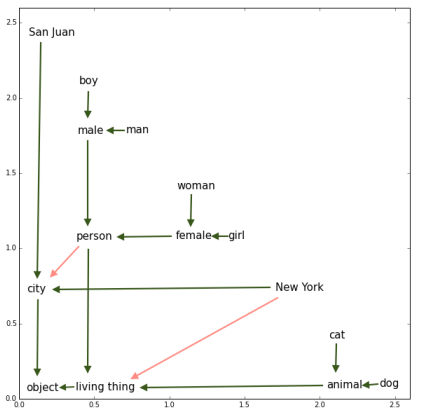
\includegraphics[width=.8\linewidth]{img/emb-orderemb.png}  
          \caption{\textit{Order Embeddings}}
          \label{subfig:orderemb}
    \end{subfigure}
    \begin{subfigure}{.33\textwidth}
          \centering
          % include first image
          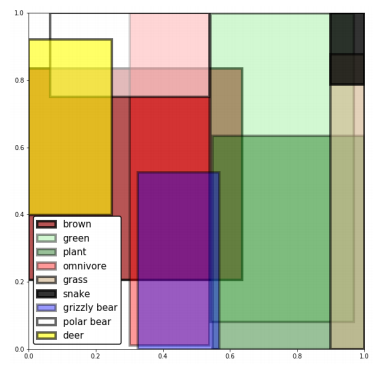
\includegraphics[width=.8\linewidth]{img/emb-boxlattice.png}  
          \caption{\textit{Box-Lattice Embeddings}}
          \label{subfig:boxlatticeemb}
    \end{subfigure}
    \begin{subfigure}{.33\textwidth}
          \centering
          % include first image
          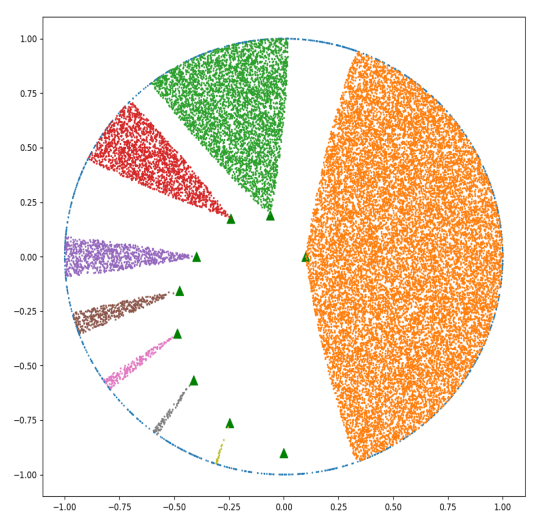
\includegraphics[width=.8\linewidth]{img/emb-poincone.png}  
          \caption{Plongements de Poincaré}
          \label{subfig:poincone}
    \end{subfigure}
    \caption[Plongements lexicaux spécifiques à l'hyperonymie]{(brouillon) Zones d'hyponymies pour  différents modèles de plongement lexical utilisés pour la détection d'hyperonymes. La zone d'hyponymie associée à un concept contient tous les hyponymes de ce concept.}
    \label{fig:litt-emb-models}
\end{figure}


\iffalse {
Une paire de mots $(x_k, y_k)$ est représentée par la différence entre ses plongements $\textbf{x}_k - \textbf{y}_k$ : 


\cite{fu2014learning} utilise des plongements lexicaux généralistes et entraînent ensuite un classifieur capable d'identifier les relations d'hyperonymie à partir de ces plongements; à l'inverse \cite{}

en combinant les représentations de A et de B et en calculant un score.

Les méthodes distributionnelles s'appuyent sur des plongements lexicaux tels que \cite{mikolov2013distributed} pour obtenir des représentations riches des mots d'un corpus, et évalue ensuite si une paire de mots correspond à une relation d'hyperonymie à l'aide d'une fonction de score qui dépende des plongements de ces mots. Elles reposent sur l'«hypothèse d'inclusion distributionnelle» (ou \textit{Distributional Inclusion Hypothesis}) \cite{geffet2005distributional} : si A est un hyperonyme de B, alors les contextes dans lesquels B apparaît forment un sous-ensemble des contextes dans lesquels A apparaît. Intuitivement, cela signifie que l'on peut remplacer les occurrences de B par A tout en gardant un texte valide.

Une méthode distributionnelle repose donc sur (a) une méthode de plongement lexicale, capable d'obtenir des représentations denses et de faible dimension des mots; (b) une fonction de classification, qui combine les plongements de deux mots et évalue si le premier mot est un hyperonyme du second. 
%De nombreuses méthodes existent, selon des plongements 
% Class-based

% HyperVec
% Poincaré Embeddings

% Autres approches :
% Ontology Completion Using Graph Convolutional Networks
% Petrucci & Rospocher
}
\fi 

% TIEmb / NICKEL
% TaxoGen
% Gupta ?
% Petrucci, Rospocher
% GCN Li/Bouraoui



\subsubsection{Regroupement hiérarchique sur les plongements lexicaux}


Il existe une proximité naturelle entre un arbre de clustering hiérarchique et une taxonomie, si bien qu'il est naturel d'appliquer, comme nous le faisons dans ce mémoire, un algorithme de regroupement hiérarchique à des plongements vectoriels (qu'ils soient lexicaux ou non) dans le but d'obtenir une taxonomie.  De nombreuses méthodes ont été proposées dans ce sens, que l'on détaille dans les lignes qui suivent. On verra que chacune présente des différentes majeurs avec l'approche que nous proposons.


En premier lieu, la majorité des méthodes fonctionne au niveau des concepts, et non au niveau des instances.
% TaxoGen
% Gupta
% Bayesian Rose Tree (Blundell, Song)


\section{Regroupement hiérarchique sur les graphes}
